\documentclass[onecolumn,10pt,cleanfoot]{asme2ej}

\usepackage{graphicx} %% for loading jpg figures
\usepackage{bm}
\usepackage{nicefrac}
\usepackage{mathtools}
\usepackage{amssymb}
\usepackage{amsmath}
\usepackage{parskip}
\usepackage{listings}
\usepackage{tablefootnote}
\usepackage{float}
\usepackage{xcolor}
\usepackage{xurl}

%%% first author
\author{Jonatan H. Hanssen
    \affiliation{
	Bachelor Student, Robotics and \\
	Intelligent Systems\\ \\[-10pt]
	Department of Informatics\\ \\[-10pt]
	The faculty of Mathematics and \\
	Natural Sciences\\ \\[-10pt]
    Email: jonatahh@ifi.uio.no
    }
}

\author{Eric E. Reber
    \affiliation{
	Bachelor Student, Robotics and \\
	Intelligent Systems\\ \\[-10pt]
	Department of Informatics\\ \\[-10pt]
	The faculty of Mathematics and \\
	Natural Sciences\\ \\[-10pt]
    Email: ericer@ifi.uio.no
    }
}

\author{Gregor Kajda
    \affiliation{
	Bachelor Student, Robotics and \\
	Intelligent Systems\\ \\[-10pt]
	Department of Informatics\\ \\[-10pt]
	The faculty of Mathematics and \\
	Natural Sciences\\ \\[-10pt]
    Email: grzegork@ifi.uio.no
    }
}

\begin{document}

\title{Hybrid models as an alternative to Convolutional Neural Networks for image classification}

\maketitle

\section{Abstract}

We compared convolutional neural networks, the de facto standard for image classification problems, with hybrid models created by combining neural networks with principal component analysis (PCA) and random forests (RF). By doing this, we explored the tradeoff between prediction accuracy and computational cost for four different ML models: A pure CNN model, a CNN-RF model, a PCA-NN model and a PCA-RF model. We used these models on the well known MNIST dataset and the Guangzhou pneumonia dataset consisting of x-ray images of potential cases of pneumonia. From this, we found that pure CNNs performed best in terms of accuracy, achieving test accuracies of $99.0\%$ and $88.8\%$ on the MNIST and pneumonia dataset, respectively. However, we found that the PCA-NN model performed similarly, at a much lower computational cost, achieving an impressive $88\%$ increase in prediction speed at the cost of only $1.1$ percentage points in accuracy.

\section{Introduction}

The task of image recognition and classification is a great challenge in machine learning, as there are a large number of features present in the data which slow down our training and prediction speed. For a relatively small one-channel image of $227$ by $227$ pixels, the naive approach of using every pixel as a feature becomes unfeasable, as we now have $51$ thousand features. Clearly, some form of dimension reduction must be used to rectify this problem, and Convolutional Neural Networks (CNNs) are regarded as the gold standard for this. CNNs are able to reduce the dimensionality while extracting useful information in each layer, for example by finding edges in the first layer, combinations of edges that make a shape in the next layer, and combinations of shapes that resemble an object in the last layer. However, all these layers of convolution introduce significant computational costs, and CNNs are often reliant on graphical processing units (GPUs) for efficient training and prediction. In many embedded systems or mobile devices, the computational cost introduced by using deep CNNs may not be ideal, as the absence of dedicated hardware may lead to long prediction times. Furthermore, these systems may have real-time constraints, needing to make many predictions per second. In this paper, we explore alternative models for image classification, using principal component analysis and random forests in combination with parts of the pure CNN model. We will investigate how these architectures perform for a simple image classification problem such as the MNIST dataset, as well as a more difficult classification problem in the form of pneumonia prediction from X-ray images. 

More specifically, we will compare four different architectures. First we will use a pure CNN, where a series convolutional layers\footnote{We follow the terminology used in Goodfellow et Al. \cite[336]{gbc}, where what is denoted as a single convolutional layer includes the convolutional, detector and pooling stage} is followed by a series of fully connected layers. We will then modify our CNN to create a hybrid CNN-RF model, where the features extracted by the CNN are fed into a random forest, which makes the final prediction. Finally, we will make use of principal component analysis instead of convolution and pooling for dimensionality reduction, feeding the results of this stage into either a neural network or a random forest. In doing this, we hope to answer the following question: could hybrid models be a viable alternative to CNNs, either by directly outperforming them in accuracy, or by offering an appealing tradeoff between performance and computational effort?

First, we will give an explanation of the theory and method used in this paper, followed up with a detailed discussion of our results. Finally, we will arrive at a conclusion which summarizes our core results and lessons.

\section{Method}

\subsection{Theory}

This sections covers the theoretic background which underlies the methods used in this paper.

\subsubsection{Convolutional Neural Networks}

Convolutional Neural Networks are neural networks which are specialized to work on images, or other types of data where the structure of the data carries meaning. A normal neural network treats each input independently, and inputs are flattened such that any spatial information is lost. CNNs, on the other hand, explicitly take the spatial dimensions into account, by using convolutional kernels and pooling layers as part of their architecture.

The eponymous operation of convolution is a method which is often used in image processing. It is performed by using a convolutional kernel, which is applied to each pixel of the image. The kernel is a matrix of values, and the output of a particular pixel is the sum of all the pixels in its neighbourhood multiplied by the overlapping value in the kernel. As such, the value in any one position is dependent on the kernel, but also on the pixels around this position. This allows us to extract valuable information about images, such as edges or patterns. A basic kernel could be the Laplacian kernel (Eq.~\ref{laplace}), which will output a high value when the pixel in the middle of the kernel has a value which differs greatly from the pixels in a 3 by 3 neighbourhood around it. As such, this kernel can be used to detect edges, as edges imply large local changes in pixel intensity. The effect of this kernel can be seen in figure ~\ref{millie}.

\begin{equation}
\label{laplace}
laplace : 
\begin{bmatrix}
-1 & -1 & -1 \\
-1 & 8 & -1 \\
-1 & -1 & -1
\end{bmatrix}.
\end{equation}

\begin{figure}[H]
\centerline{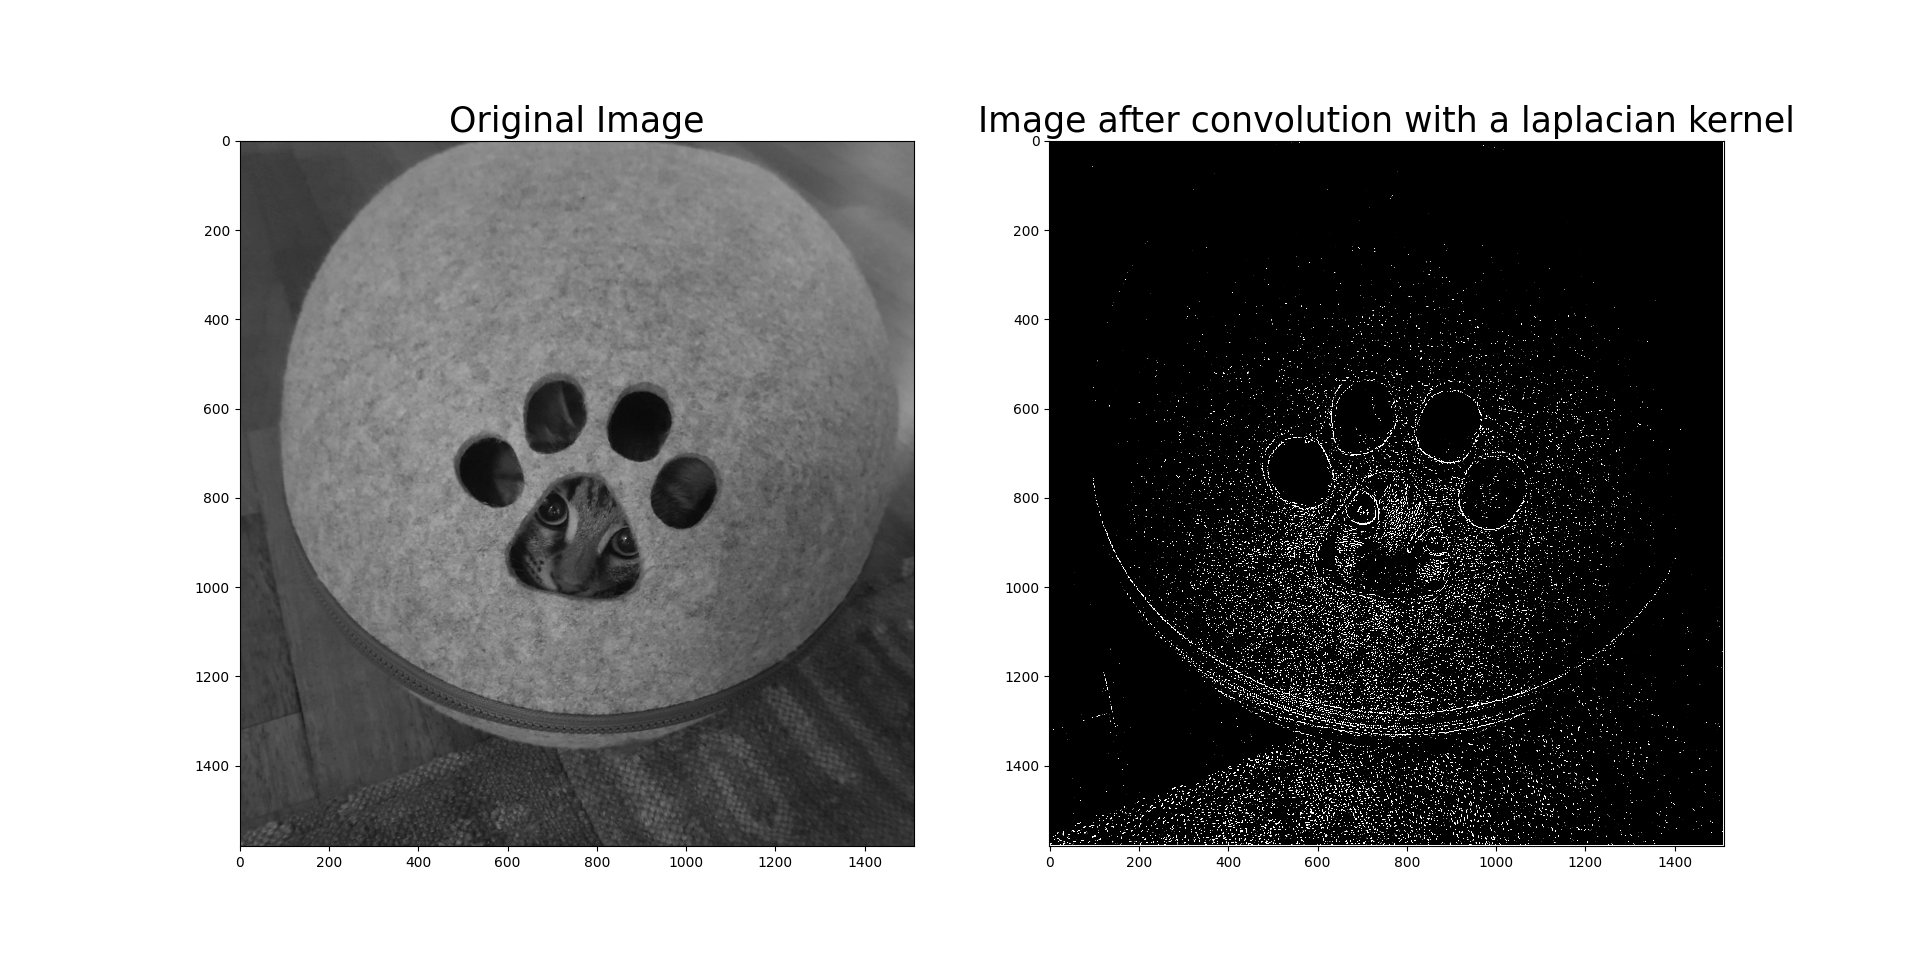
\includegraphics[width=8in]{figure/millie.png}}
\caption{The result of applying the kernel in Eq.~\ref{laplace} to an image. Here we can see that areas of relatively constant intensity disappear (the floor, the back part of the box), while sharp edges elicit a response (the transition between carpet and floor, the holes in the box). However, a lot of noise is also present. This can be solved with more sophisticated methods of edge detection, such as Canny's algorithm.}
\label{millie}
\end{figure}

The mathematical equation for the convolution of a kernel $w$ on an image $f(x,y)$ (represented as a discrete function in two variables) is as follows\footnote{In reality, we should have $x-s$ and $y-t$, as convolution involves rotating the kernel by 180 degrees. However, the term convolution is often used for both the mathematical operations of correlation and convolution\cite[160]{dip}. Furthermore, the kernels used in CNNs have randomly initialized weights, making rotation inconsequential.}:

\begin{equation}
w \star f(x,y) = \sum^a_{s=-a} \sum^b_{t=-b}f(x+s, y+t).
\end{equation}

In a convolutional neural network, the values of each kernel are initialized randomly, and training involves tuning these values. When performing convolution at the edges of an image, some values in the image will be undefined (i.e, some values of the kernel will not overlap with the image). To solve this problem, we can either ignore any positions where the kernel is not fully contained within the image, or introduce padding, where we pad the image with values (usually just zeroes) so that more of the image can be convolved. By choosing the amount of padding, we can decide how close the dimensions of the result of our convolution are to the original dimensions. Another parameter which has an effect on the output dimensions is the {\it stride} parameter, which decides the size of the step between each convolution operation. By having a stride higher than one, we are no longer evaluating at every position. This reduces the computational complexity at the cost of not extracting our features as finely \cite[343]{gbc}. This will also downsample the result of our convolution to a smaller dimension than the input.

The convolution stage is often followed by an activation function, like the RELU function. After this, it is common to use a {\it pooling layer}. This layer replaces the output at a certain location with a summary statistic of the nearby outputs \cite[335]{gbc}. We could for example replace the value at a given position with the maximum value in a neighbourhood around this position, which is known as {\it max pooling}. By using pooling, we are making our output invariant to small translations of the input. This is useful if we care more about whether a feature is present rather than exactly where it is \cite[336]{gbc}. Furthermore, by using a stride parameter here as well, we are able to downsample our output.

After several layers of convolution, the input has usually been downsampled, and important features about the input have hopefully been extracted by the use of convolution and pooling. The output is then flattened, and the features are sent to one or more fully connected layers. The outputs of these layers are then used to make a prediction.


\subsubsection{Principal Component Analysis}

Principal Component Analysis is a dimensionality reduction method which projects our dataset onto a lower dimension, while capturing as much of the variance of our data as possible. The central idea is to change the basis we use to represent our dataset, using vectors pointing in the principal directions of our dataset, instead of the unit vectors in feature space. The principal directions point in the direction of the variance of our dataset. By simply changing our basis to these vectors, called principal components, we have not achieved any dimensionality reduction, but by discarding directions of very little variance, we can reduce dimensionality without losing much variance (and thus information). By performing a Singular Value Decomposition we have everything we need to achieve this. The SVD is as follows:

\begin{equation}
X = UDV^T
\end{equation}

Here, the coloumns of $U$ are known as the left singular vectors of $X$, $D$ is a diagonal matrix containing the singular values of $X$ (the square roots of the eigenvalues of $X^TX$) and the coloumns of $V$ are known as the right singular values. The right singular values are actually the principal components we need, ordered by the variance in that direction. Thus, we can project our dataset down to a subspace spanned by a subset of these vectors (for example the first 3 vectors) and reduce the dimensionality of our dataset while losing as little information as possible. Furthermore, the coloumn vectors of $V$ are orthogonal, and as such we can project our dataset down to this subspace with a single matrix multiplication:

\begin{equation}
\hat{X} = XV
\end{equation}

For very large design matrices, the computational complexity of calculating the singular value decomposition can be significant. However, there exists stochastic methods to achieve good approximations, like Randomized PCA \cite[227]{halko}. Furthermore, when a decomposition is found, transforming any arbitrary input is trivial.

\subsubsection{Decision Trees}

A decision tree is an intiutive way of performing both classification and regression tasks, by asking a series of yes or no questions about an instance in the dataset. These questions will split the original dataset, the root node, into child nodes which contain subsets of the dataset, and these nodes will be split again, creating a tree structure which terminates in leaf nodes which imply a choice of class.

For classification problems, the algorithm for creating a decision tree is quite simple. First, consider each feature of the dataset, and attempt to split all instances into two child nodes based on a simple true/false statement about this feature. Having done this for every feature, calculate the degree of homogeneity\footnote{This can described by calculating the Gini-factor, or by calculating the entropy of the set} of the two child nodes created, when considering the actual class of the instances. The feature which created the most homegenous split, is the feature which has the largest effect on the final class, and as such should be the first feature we use to split the dataset. After this, we have two subsets, and we perform the same algorithm on these subsets again. This algorithm terminates when it is not possible to split the data further, because all nodes only contain instances belonging to the same class. In practice, it is advised to stop the algorithm earlier by introducing limits to the depth of the tree, or limits to how few instances can be in one node. Once the algorithm has terminated, we have a series of leaf nodes containing subsets of the data.

Once a tree has been built, prediction is done by taking the instance and propagating it down the tree by answering the true/false statements that have been decided on in the creation of the tree. Once we have reached a leaf node, we predict that this instance is the class to which the majority of the instances in the leaf node belong to.

Decision trees are intuitive and computationally cheap to create, not requiring any training due to the deterministic nature of the algorithm. Furthermore, they require little tuning and have few hyperparameters. However, they are prone to overfitting.

\subsubsection{Random Forests}

A Random Forest is a type of ensemble method used to improve the performance of a single decision tree, by using bagging. Instead of using a single tree, a random forest consists of many similar trees, and the final class is determined by majority voting by all the trees. Like decision trees, they are relatively simple to understand.

To create a random forest, we perform a bootstrap of the original dataset, creating many similar instances with small permutations introduced by resampling with replacement. We now create one decision tree per bootstrap, only using a random subset of the total amount of features every time we perform a split\footnote{The number of features used is often set to $\sqrt{p}$, where $p$ is the number of features in the dataset}. The result of this is that we create many slightly different trees. These trees give predictions which are worse than simply creating a single decision tree using all the features and all the data, but when basing our prediction on the majority vote of all the trees, we are able to make predictions which are more generalizable and less prone to overfitting.

\subsubsection{Datasets}

Below is a description of each of the datasets used in this report.

\subsubsection{MNIST}

The MNIST dataset is a well known multiclass classification problem used to test machine learning algorithms. It consists of $70000$ black and white images of hand drawn digits, each $28$ by $28$ pixels. Each image is labeled with one of ten classes, corresponding to the digit it depicts. The dataset is divided into $60000$ training images and $10000$ test images. This dataset is essentially uniformly distributed, with all classes containing around $9 - 11\%$ of the total dataset.

\subsubsection{Guangzhou Chest X-Ray Pneumonia Dataset}

The Guangzhou Chest X-Ray Pneumonia Dataset consists of $5856$ X-Ray images of children between the ages of one to five. The images were taken from the Woman and Children's Medical Center in Guangzhou, China. The dataset is divided into a training set of $5232$ images and $624$ test images. The dataset is not evenly distributed, having $74.2\%$ instances of pneumonia in the training set and $62.5\%$ instances of pneumonia in the testing set. The data was collected and labeled as a part of the article {\it Identifying Medical Diagnoses and Treatable Diseases by Image-Based Deep Learning}, published in {\it Cell} \cite{xray}.

\subsection{Implementation}

Our implementation can be found at \texttt{github.com/Gregz9/CNN\_vs\_weak.git}.

All neural network stages were implemented through the Keras API, using the Tensorflow library. Randomized PCA was implemented using Scikit-learn's PCA class, which follows the algorithm of Halko et Al.. Random Forests were implemented using the Tensorflow Decision Forests library. For hyperparameter tuning, we used the Keras Tuner library \cite{kerastuner}. For the CNN-RF model, we extract the outputs of the final hidden layer of the CNN per instance in the dataset, and use this as inputs to the random forest.

\section{Results}

With the theory and implementation explained, we can now discuss the results we achieved by applying these methods.

\subsection{MNIST}

To test our hybrid models against a pure CNN model, we applied them all to the MNIST dataset.

\subsubsection{Traditional Convolutional Neural Network}

As is well known, convolutional neural networks perform excellent on the MNIST dataset, achieving test accuracies rivaling humans. As an initial guess for the architecture, we used only a single convolutional layer followed by a dense layer. The convolutional layer had $32$ filters. By gridsearch, we found the optimal filter width to be $7$ and the optimal learning rate to be $0.001$. With these hyperparameters we achieved a test accuracy of $99.0\%$, a very good result. Furthermore, we acieved a recall of NUMBER and precision of NUMBER. Based on this result, we conclude that no more hidden layers or regularization parameters need to be included. Looking at the heatmap (Fig.~\ref{mnistheatmap_cnn}), we can see that our predictions are excellent in all classes, never misclassifying any single class more than $2.4\%$ of the time.

\begin{figure}[H]
\centerline{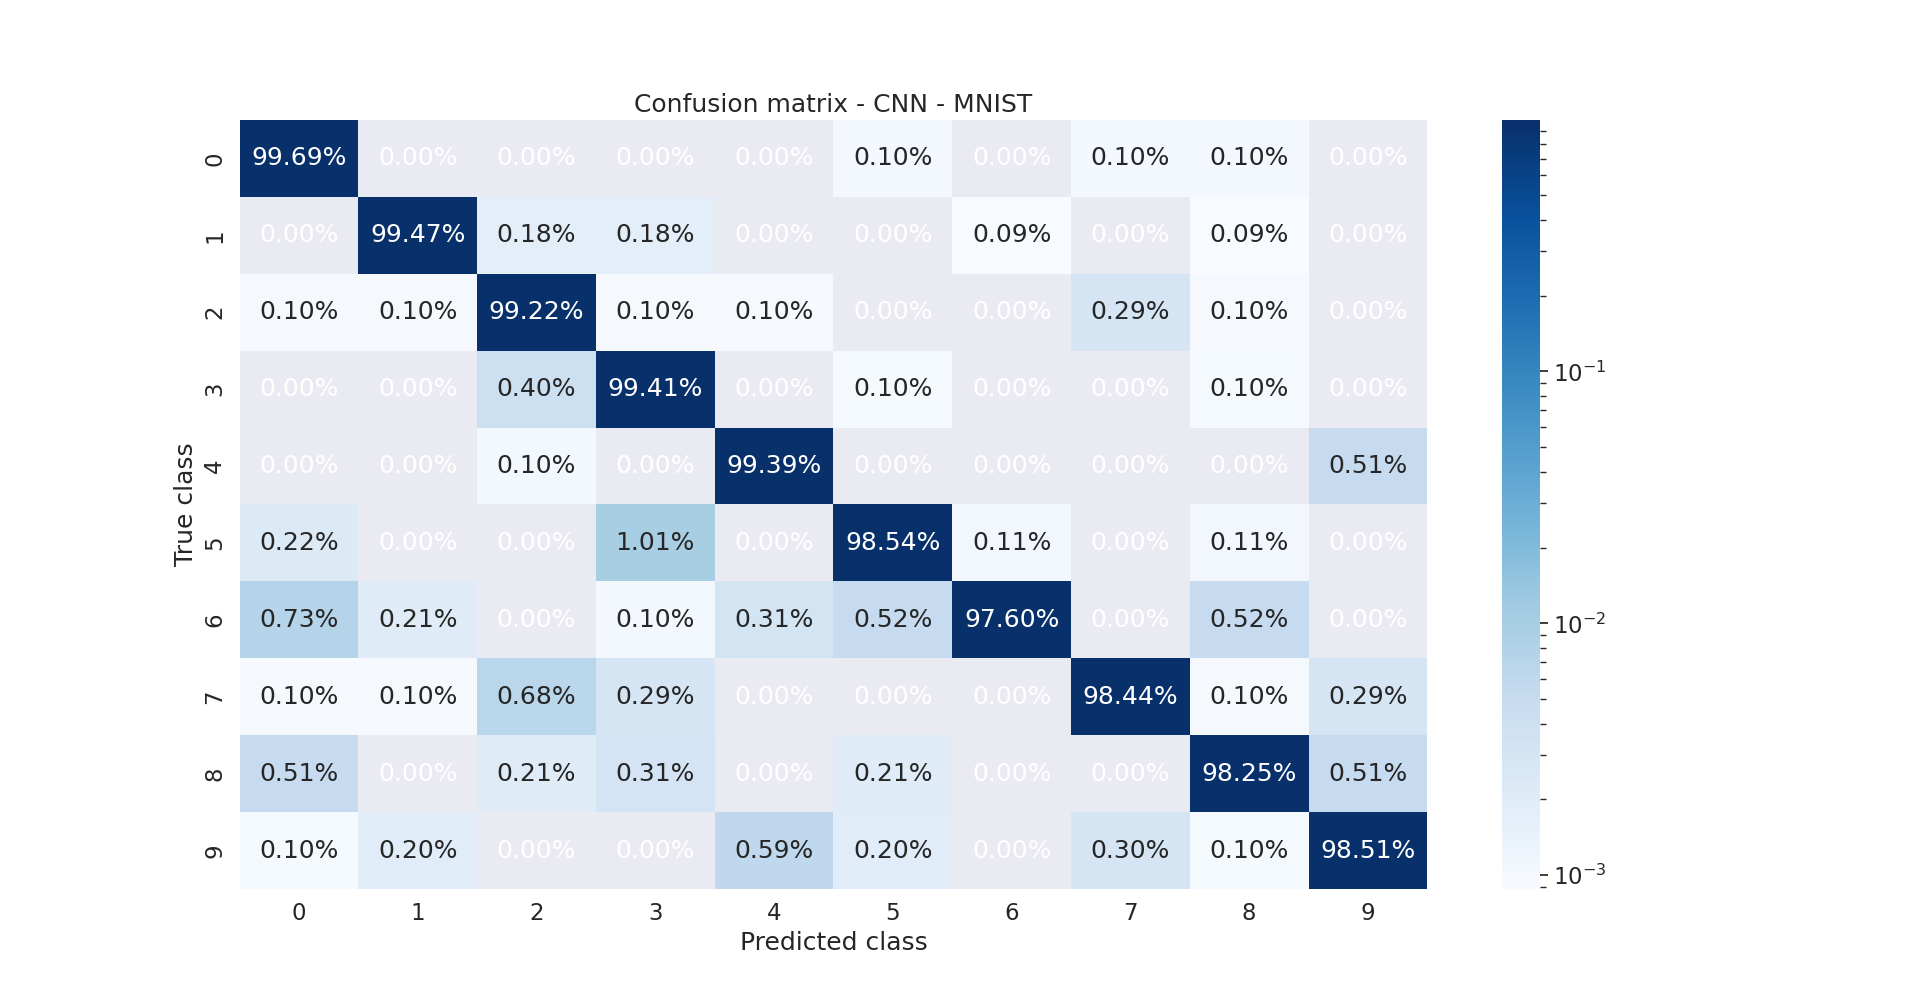
\includegraphics[width=8in]{figure/conf_cnn_MNIST.png}}
\caption{Confusion matrix for MNIST dataset classified using a CNN. From this figure, we can see that most misclassifications occur for digits that look similar: eights are sometimes misidentified as zeroes, and fours and nines are sometimes misidentified as eachother.}
\label{mnistheatmap_cnn}
\end{figure}

\subsubsection{Convolution followed by a Random Forest}

Given that we have achieved excellent results by using a CNN, we may not expect to achieve better results by sending the extracted features to a random forest. Regardless, we found that by using the same CNN model we found previously, and sending the extracted features into a random forest model, we achieved a testing accuracy of $98.9\%$, which is essentially equivalent to our pure CNN model. Furthermore, this method introduced a significant computational cost to the prediction, as can be seen from table~\ref{modcompmnist}. From this we conclude that a CNN-RF hybrid model is inferior to a pure CNN model in this case, achieving both lower accuracies and being more computationally expensive.

\subsubsection{Principal Component Analysis followed by a Neural Network}

With somewhat disappointing results from introducing a different model when making the prediction, we instead attempt to perform the feature extraction and dimensionality reduction stage with a different method. We therefore attempt to use Principal Component Analysis, and can see that we are able to reduce the dimensionality of our dataset while retaining a large amount of the information. Looking at figure~\ref{pcacomp}, we can see that even when using only the $50$ first principal components, the numbers are still readable. This implies that we are able to reduce the amount of features we send to the dense layers and still expect reasonable results.

\begin{figure}[H]
\centerline{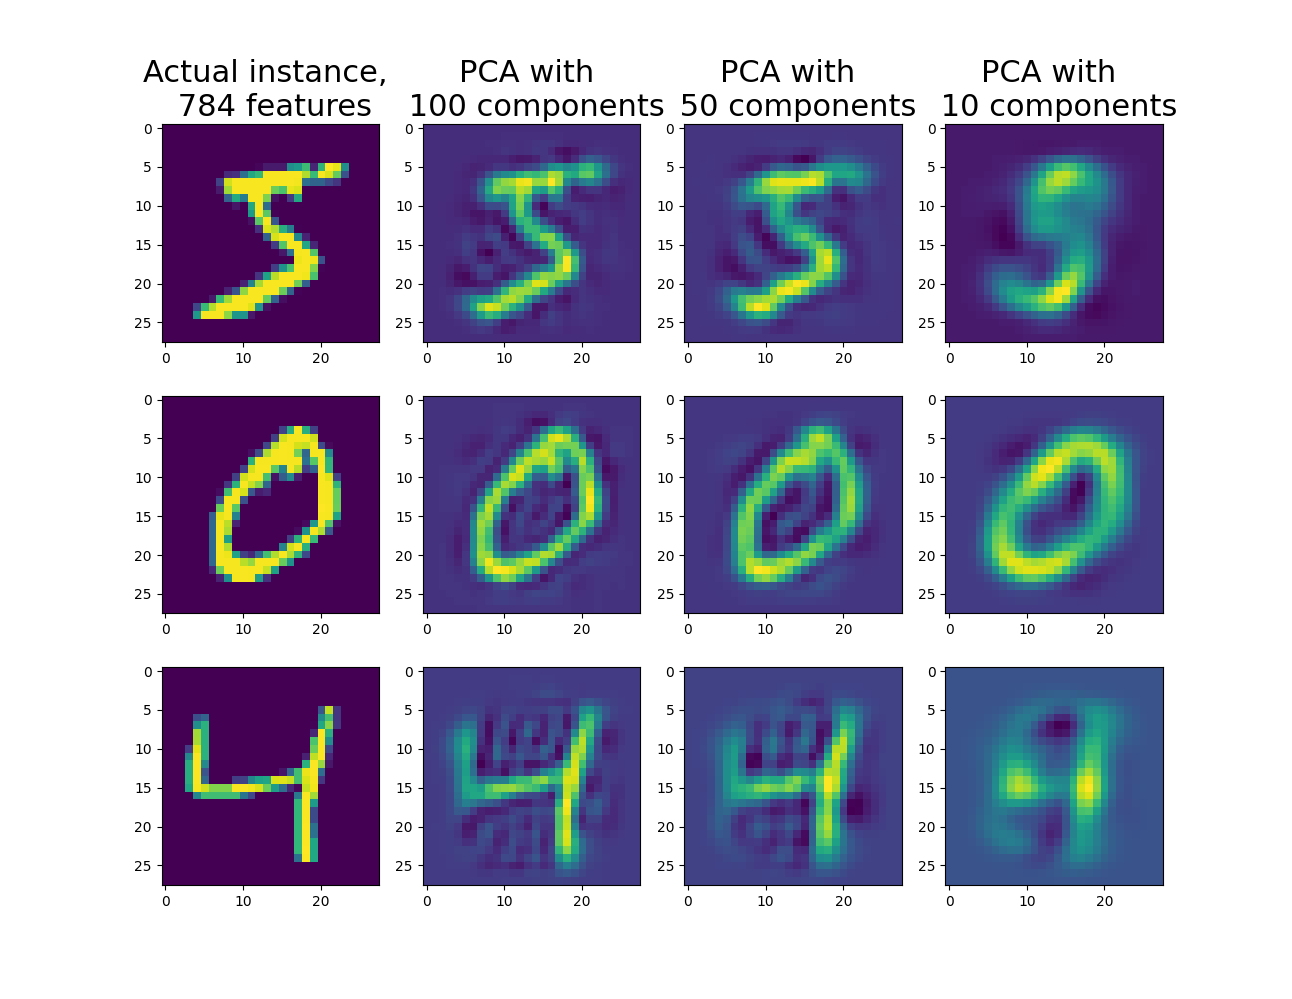
\includegraphics[width=5in]{figure/pcacomp.png}}
\caption{Comparison showing the amount of information lost by reducing the amount of principal components}
\label{pcacomp}
\end{figure}

Using different amount of principal components, we sent the reduced dataset into a neural network with three hidden layers. After testing different amounts of principal components to keep, and tuning the hyperparameters based on these, we found that even with only $50$ principal components, we achieved a test accuracy of $98.1\%$, a recall of NUMBER and a precision of NUMBER. This was achieved with $224$ nodes per layer and a learning rate of $0.001$. These results are comparable to the accuracy obtained by a convolutional neural network. Looking at figure~\ref{mnistheatmap_pcann}, we again see that we are making accurate predictions across all classes. Furthermore, when looking at the speed at which we are able to make predictions, we see that this model makes predictions around $34\%$ faster than a pure CNN model, while sacrificing less than a single percentage point in accuracy. However, when using a GPU, there is very little difference in prediction time between the two models. Regardless, this decrease in computational effort could offer an appealing tradeoff for embedded systems which do not have access to dedicated GPUs.

\begin{table}[H]
\caption{Optimal hyperparameters for the PCA-NN model}
\begin{center}
\label{pcanntable}
\begin{tabular}{| l | l | l | l |}
\hline
Principal Components & Nodes per hidden layer & Learning Rate & Lambda \\
\hline
9 & 9 & 0.1 & 0.0001 \\
\hline
\end{tabular}
\end{center}
\end{table}

\begin{figure}[H]
\centerline{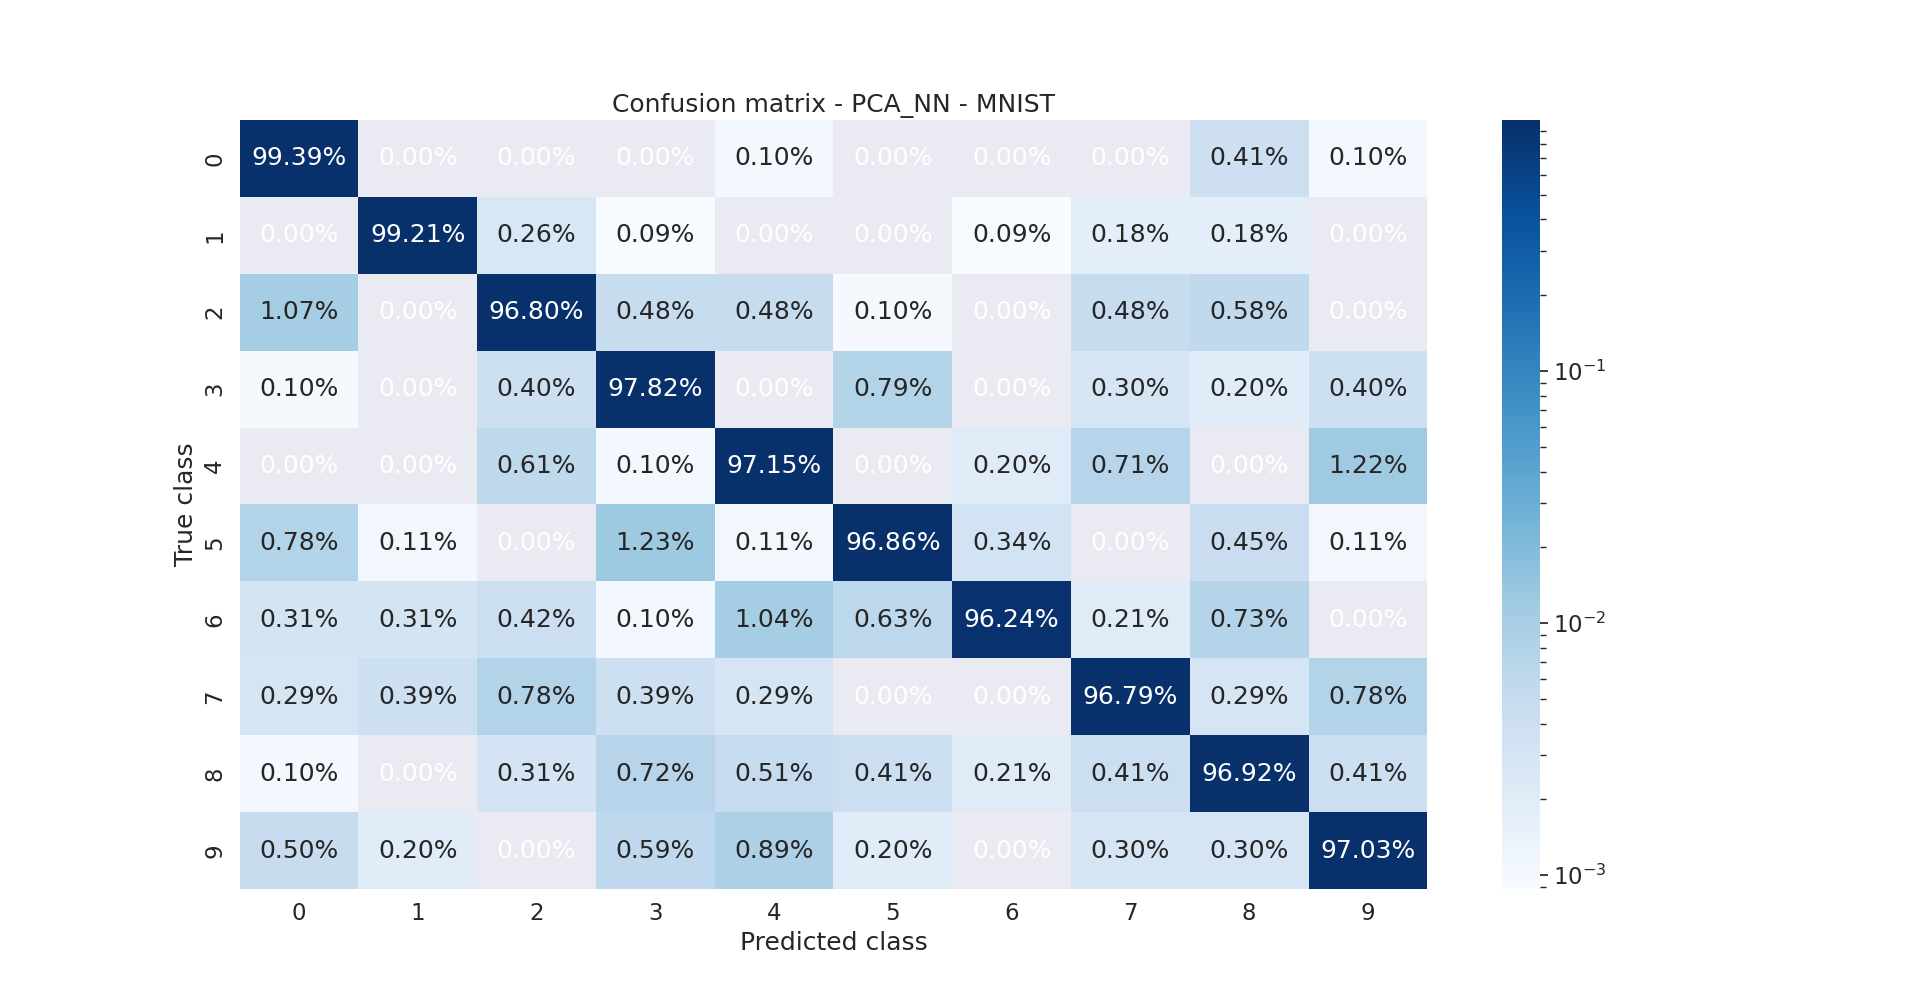
\includegraphics[width=8in]{figure/conf_pca_nn_MNIST.png}}
\caption{Confusion matrix for MNIST dataset classified using PCA followed by a neural network. Here we can see that misclassifications are slightly more common than when using a CNN, but the results are still good.}
\label{mnistheatmap_pcann}
\end{figure}


\subsubsection{Principal Component Analysis followed by a Random Forest}

Satisfied with the results achieved by replacing the convolutional stage with Principal Component Analysis, we attempt to sidestep neural networks all together, and use PCA followed by a random forest. Here, we achieved a reasonable result of $94.8\%$ accuracy on the test set. Although this is not as impressive as the previous models, it shows that decent results can be achieved without using neural networks at all. Furthermore, we again see a slight performance gain in our prediction, with this model being $38\%$ faster than the pure CNN model at making a prediction for the entire test dataset. However, the decrease in accuracy makes this tradeoff less appealing, and because the libraries we use do not offer GPU accelaration when using PCA or random forests, there is no reason to use this model when a GPU is available.

\subsubsection{MNIST model comparison}

With each model optimized and tested, we can compare them to eachother in terms of accuracy and prediction speed. Table~\ref{modcompmnist} shows the relevant values for each model. From this we can gain several insights. Firstly, we can see that we have not been able to outperform a pure CNN model with any of our hybrid models. This is not so surprising, as CNNs are regarded as the gold standard for image classification, for a multitude of reasons. However, we can also see that we are able to perform decently with all of our models, achieving test accuracies above $98\%$ for all models except the PCA-RF model, which achieved a test accuracy of $94.8\%$, a result that is still reasonable. Furthermore, both the PCA models were faster than the pure CNN model (without GPU acceleration), with the PCA-NN model presenting particularly appealing performance/cost-tradeoff.

\begin{table}[H]
\caption{Table showing the accuracy and average time used to make a prediction on the entire MNIST test dataset, for each model. All models have been tested on the same system, and the average speed is calculated over 5 predictions. Neither PCA nor RF utilize the GPU, and thus it is not possible to accelerate the PCA-RF model.}
\begin{center}
\label{modcompmnist}
\begin{tabular}{| c | l | l | l |}
\hline
Model & Test accuracy & Average prediction time & Avg. time when GPU accerelated \\
\hline
CNN & 99.0\% & 1.877s & 0.2895s \\
CNN-RF & 98.9\% & 4.910s & 4.898s \\
PCA-NN & 98.1\% & 1.244 & 0.3073s \\
PCA-RF & 94.8\% & 1.182s & - \\
\hline
\end{tabular}
\end{center}
\end{table}

\subsection{Guangzhou Pneumonia Data}

As previously stated, the Guangzhou Pneumonia Dataset was collected and labeled as part of the article {\it Identifying Medical Diagnoses and Treatable Diseases by Image-Based Deep Learning}. In this article, the authors used transfer learning using a network previously trained on ImageNet to classify the x-ray images. With this method, they achieved a test accuracy of $92.8\%$ \cite[1127]{xray}. We now turn our attention to this dataset, and see if we can achieve similar results using our methods.

\subsubsection{Traditional Convolutional Neural Network}

Determining whether an x-ray shows a case of pneumonia or not is clearly a much more difficult classification problem than our previous dataset. Therefore, we initially had problems designing an architecture which achieved much higher than $80\%$ test accuracy. Clearly, we are not able to use a simple one model consisting of only one convolutional layer, like we were able to on the MNIST dataset, and designing a general convolutional neural network architecture is a very complex task. Thus, we turn to the literature, and explore models which have been proven to be effective at image recognition. Out of the architectures presented in {\it Hands-On Machine Learning with Scikit-Learn and Tensorflow} \cite{geron}, we decided to try AlexNet, which won the ILSVRC 2012 challenge. This choice of model was motivated by a few different reasons. Firstly, AlexNet is a relatively shallow network having only $11$ hidden layers. Furthermore, although more effective models have been created after 2012, many of these use more complicated architectures such as skip layers or layers which feed their outputs to all subsequent layers. AlexNet is both a relatively simple model to train using our available hardware, and a simple model to understand. Using AlexNet with the Adam optimizer, we achieved a testing accuracy of $88.9\%$, a recall of NUMBER and a precision of NUMBER. Comparing our result to those obtained by Kermany et Al. ($92.8\%$), we see that our model is a few percentage points worse. Looking at the confusion matrix (Fig.~\ref{conf_cnn_pneu}), we can also see that our model is biased, being more prone to create false positives than false negatives. This is due to the imbalance of the training dataset, which has more cases of pneumonia than not. We have used class weighting when training our model, which greatly improves upon the accuracy gained without weighting, however even with this, we are not able to remove the bias completely\footnote{That is, we have not been able to remove the bias without also severely decreasing the accuracy}. All in all, the model is worse than the one created by Kermany et Al., but when considering that we are not using transfer learning and are completing training on a single laptop, we consider our results to be reasonable.

\begin{figure}[H]
\centerline{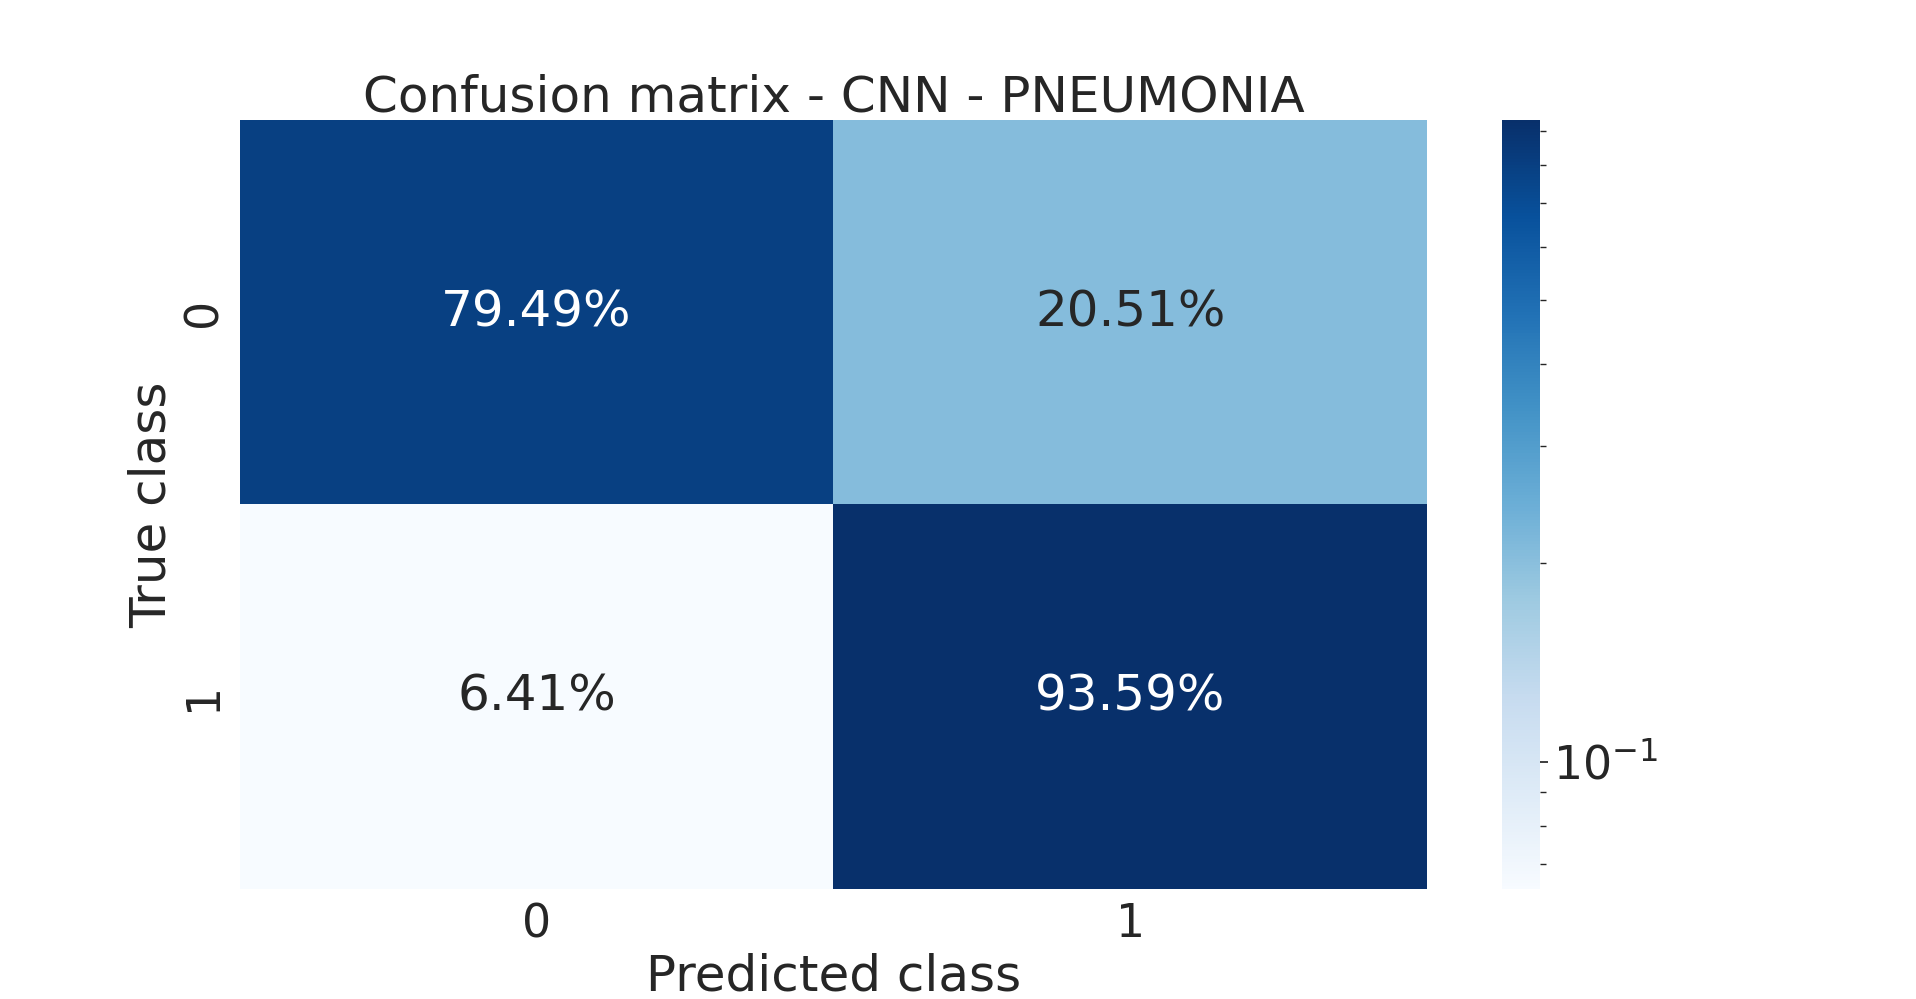
\includegraphics[width=5in]{figure/conf_cnn_pneu.png}}
\caption{Confusion matrix for the pneumonia dataset, using the CNN model}
\label{conf_cnn_pneu}
\end{figure}

\subsubsection{Convolution followed by a Random Forest}

As with the MNIST dataset, we also found disappointing results when attempting to use a CNN-RF model on this dataset. Here, we achieved a test accuracy of $88.1\%$, which is $0.7\%$ lower than simply using the CNN as is to make the prediction. Furthermore, using a random forest increases the computational complexity considerably as well, as can be seen from Table~\ref{modcomppneu}.

\subsubsection{Principal Component Analysis followed by a Neural Network}

Again, we then attempt to replace the feature extraction stage of a CNN with a simple application of Principal Component Analysis. Given the complexity of the network needed to achieve good results when using a CNN, one might not expect to find good results using PCA. However, we have found that we can actually achieve very comparable results to AlexNet using a much simpler model. In our PCA-NN model, we tried different number of principal components to keep, and sent these components into a neural network with three hidden layers. Tuning the model, we found that optimal hyperparameters were as described by Table~\ref{pcanntable}. Using these parameters, we were able to achieve a test accuracy of $87.8\%$, with a recall of NUMBER and a precision of NUMBER. This is an impressive accuracy considering the simplicity of our model, and shows that it is possible to achieve reasonable results without turning to complex convolutional neural networks. Looking at the confusion matrix, we again see a bias towards classifying images as pneumonia (Fig.~\ref{conf_pca_nn_pneu}). Regardless of the bias, we can see that the small decrease in accuracy compared to the CNN model came with a considerable gain in prediction speed when predicting using only the CPU, with the PCA-NN model being $88\%$ faster than the CNN on average (Table.~\ref{modcomppneu}). Of course, prediction of pneumonia is not a problem where one would trade accuracy for prediction speed, but there are many real-time use cases for image recognition where this is a tradeoff that is preferable.

\begin{table}[H]
\caption{Optimal hyperparameters for the PCA-NN model}
\begin{center}
\label{pcanntable}
\begin{tabular}{| l | l | l | l |}
\hline
Principal Components & Nodes per hidden layer & Learning Rate & Lambda \\
\hline
9 & 9 & 0.1 & 0.0001 \\
\hline
\end{tabular}
\end{center}
\end{table}

\begin{figure}[H]
\centerline{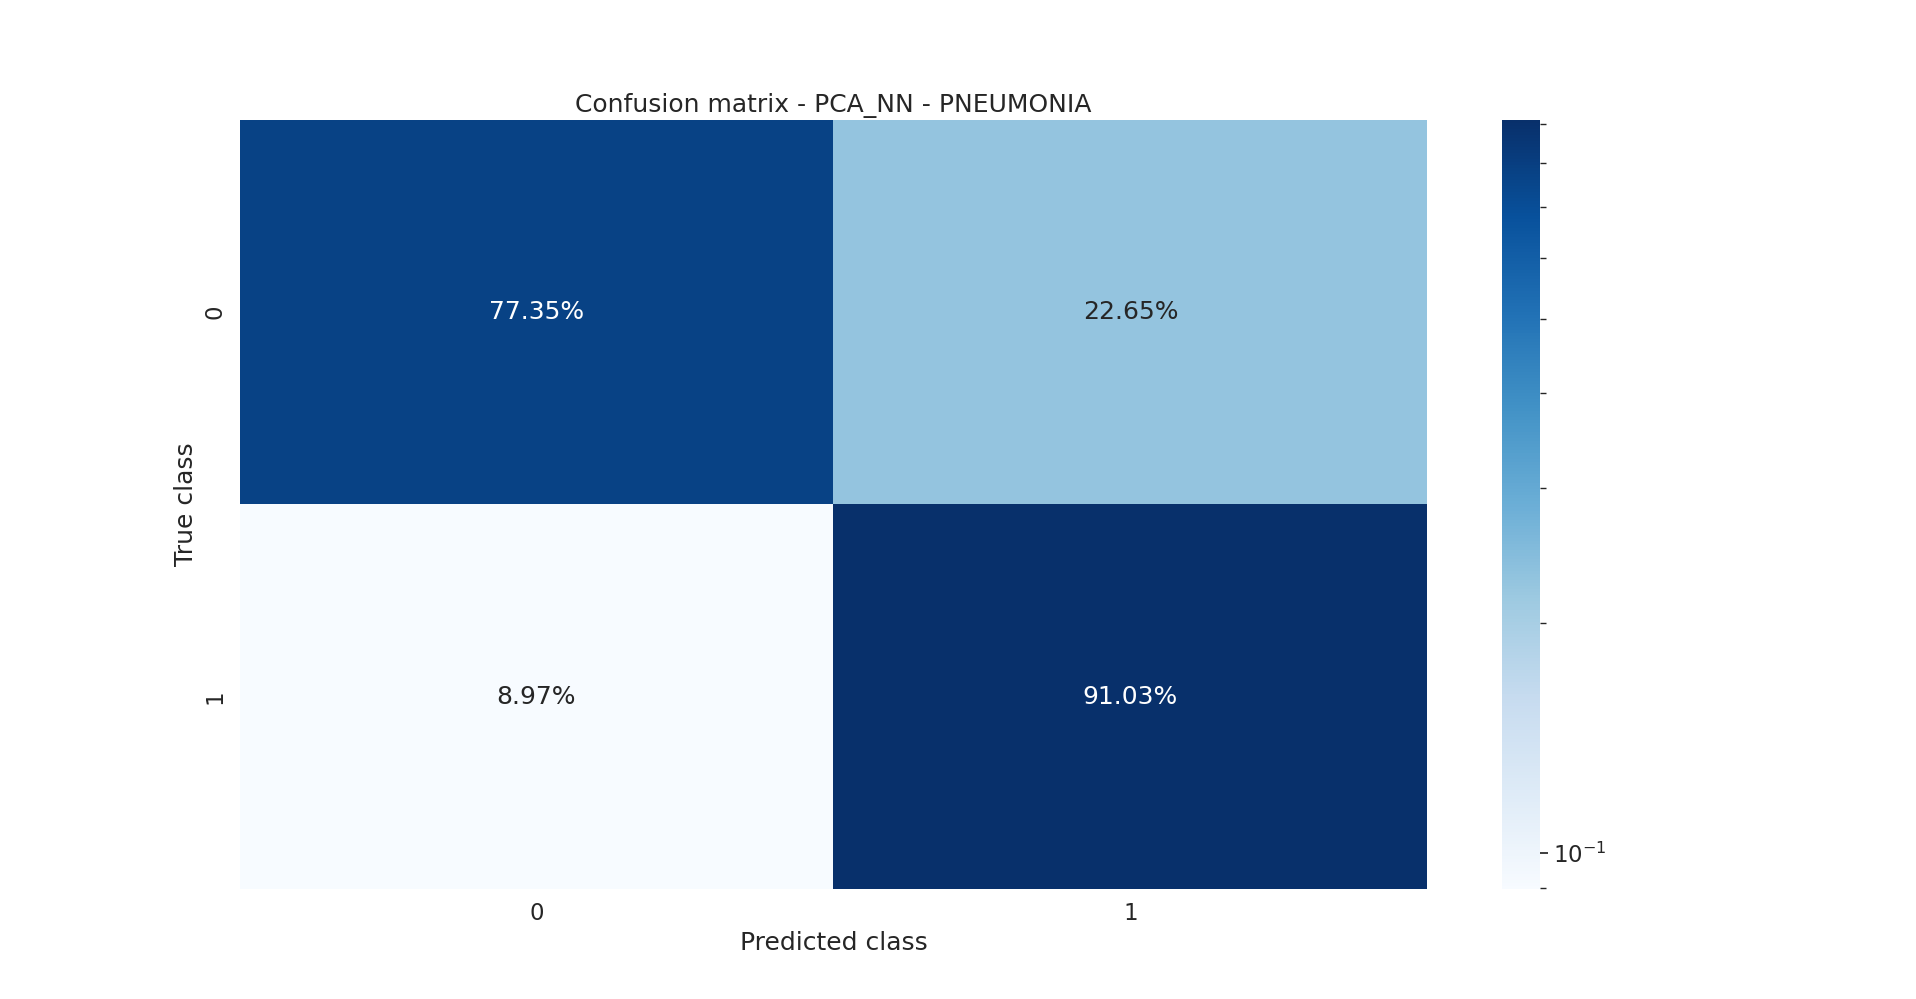
\includegraphics[width=5in]{figure/conf_pca_nn_pneu.png}}
\caption{Confusion matrix for the pneumonia dataset, using the PCA-NN model}
\label{conf_pca_nn_pneu}
\end{figure}

The fact that only $9$ components were needed is quite surprising, but could be explained by the homogeneity of the dataset. Unlike the MNIST dataset, where each class is very different, both the positive and negative classes of pneumonia have images which are very similar, as can be seen in figure~\ref{pneupcacomp}. It is then likely that the first $9$ principal components capture the variance which in large part decides whether an image displays of a case of pneumonia or not. In figure~\ref{pneupcacomp} we can also see the recreated images from the $9$ components. Although it is difficult for the human eye to differentiate the negative from the positive in these images, there is clearly enough information left, given that the model achieves the test accuracy that it does.

\begin{figure}[H]
\centerline{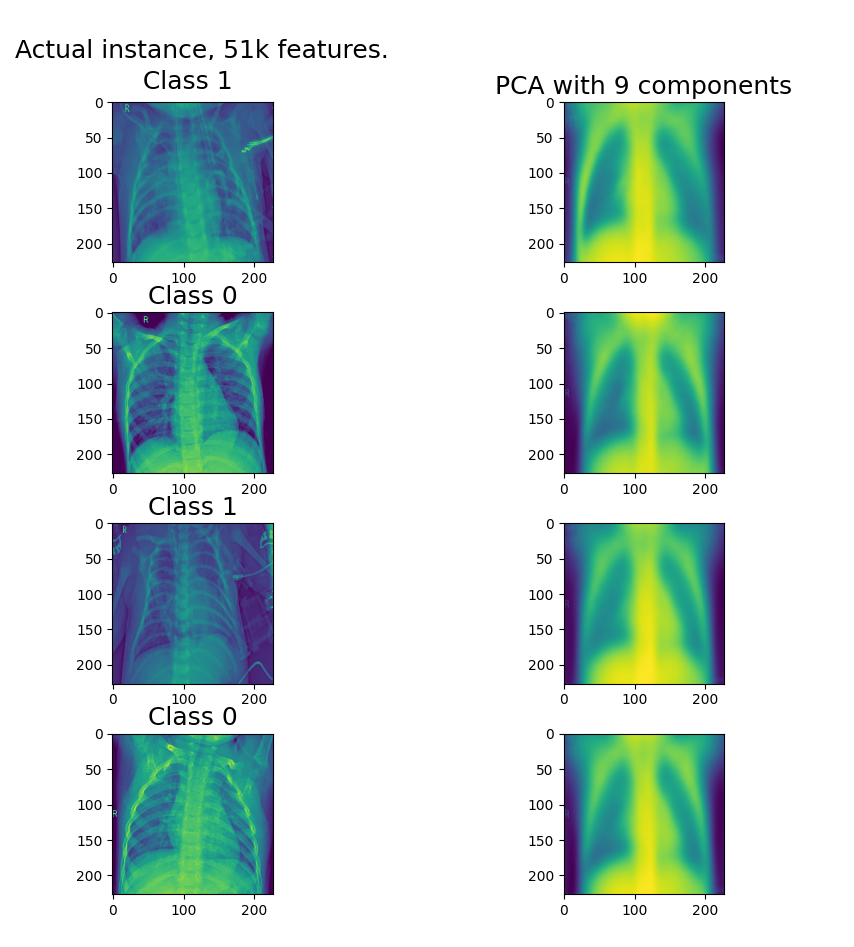
\includegraphics[width=6in]{figure/pneupcacomp.png}}
\caption{Instances from the Guangzhou dataset and their PCA reconstruction using only 9 principal components}
\label{pneupcacomp}
\end{figure}

\subsubsection{Principal Component Analysis followed by a Random Forest}

Yet again impressed with the performance of using a simpler model, we attempt to perform the same classification without using neural networks at all. Using a PCA-RF model, we achieved a test accuracy of $84.9\%$. Although this is lower than the other models, this model was by far the fastest when only a CPU, being $94\%$ faster than the CNN and $50\%$ faster than the PCA-NN model (Table.~\ref{modcomppneu}). Like with the MNIST dataset, we see that we are able to trade accuracy for performance by using simpler hybrid models to make our prediction.

\subsubsection{Pneumonia model comparison}

Having optimized all our models, we are again able to compare them against eachother in terms of accuracy and performance. Looking at table~\ref{modcomppneu}, we see much of the same story as with the MNIST dataset. We see that the pure CNN is the optimal choice when accuracy is the most important factor, and the undisputed champion in terms of both accuracy and prediction time if a GPU is available. However, when looking at CPU-prediction times, the CNN is quite slow, and the PCA-NN model makes a strong case for trading a single percentage point of accuracy for an $88\%$ increase in speed. While they cannot beat the CNN in terms of accuracy, these simpler models are an ideal fit for embedded systems with real-time constraints.

\begin{table}[H]
\caption{Table showing the accuracy and average time used to make a prediction on the entire test dataset, for each model}
\begin{center}
\label{modcomppneu}
\begin{tabular}{| c | l | l | l |}
\hline
Model & Test accuracy & Average prediction time & Avg. time when GPU accerelated \\
\hline
CNN & 88.9\% & 2.864s & 0.1179s \\
CNN-RF & 88.1\% & 3.437s & 3.356s \\
PCA-NN & 87.8\% & 0.3387s & 0.1823s \\
PCA-RF & 84.9\% & 0.1667s & - \\
\hline
\end{tabular}
\end{center}
\end{table}

\section{Conclusion}

In this paper, we have compared CNNs to different hybrid models, in an attempt to explore the accuracy/performance-tradeoff of model complexity and prediction time. We have applied four different machine learning models on the MNIST and Guangzhou Pneumonia dataset, and compared their accuracy and prediction time against eachother. In our application of these models, we found that the CNN performed best in terms of accuracy on both datasets, achieving test accuracies of $99.0\%$ and $88.8\%$ on the MNIST and Pneumonia dataset, respectively. However, we also found that the PCA-NN model performed well, achieving accuracies of $98.1\%$ and $88.1\%$ on the same datasets. Furthermore, these results were achieved at a much lower computational cost, with the PCA-NN model being $34\%$ and $88\%$ faster at making predictions for each dataset (when not using a GPU). These results make a compelling case for using simpler models when using systems which are time constrained and lacking in dedicated machine learning hardware. To explore these findings further, one could look at other combinations of machine learning models, such as Gradient Boosted Trees or Support Vector Machines. Another option would be to use more effective architectures than AlexNet, such as DenseNet, which may achieve good accuracies without incurring long prediction times.

\bibliographystyle{apalike}
\bibliography{bibliography}

\end{document}
